In this section we provide an alloy model trying to capture the main
features of the entities affected by the TS system. The model is built
defining signatures according to the class diagram and specifying
the constraints that comes out from the requirements.


\subsection{General model}


\subsubsection{Signatures, facts and functions}

\begin{lstlisting}[breaklines=true]
module myTaxiService/model

//Auxiliary signatures 
sig Date{} 
sig Time{}

sig Location{ 	
	zone: one Zone, 
}

abstract sig Passenger{} 
sig UnregisteredPassenger extends Passenger{} 
sig RegisteredPassenger extends Passenger{}

abstract sig TaxiState{} 
one sig OutOfService,Emergency extends TaxiState{} 
one sig Available, Busy, Moving extends TaxiState{}

abstract sig Taxi { 	
	driver: lone TaxiDriver, 	
	state: one TaxiState, 	
	numberOfSeats: one Int, 
}  

sig MinivanTaxi extends Taxi {} {numberOfSeats = 9} 
sig NormalTaxi extends Taxi {} {numberOfSeats = 4}

sig TaxiDriver{}

sig Request{ 	
	passenger: one Passenger, 	
	date: one Date, 	
	time: one Time, 	
	numberOfPassengers: one Int, 	
	location: one Location, 
}  {numberOfPassengers>=1}

sig ConfirmedRequest extends Request{ 	
	waitingTime: one Time, 	
	taxis: some Taxi, 
}

sig Reservation{ 	
	passenger: one RegisteredPassenger, 	
	date: one Date, 	
	time: one Time, 	
	numberOfPassengers: one Int, 	
	location: one Location, 	
	associatedRequest: one Request, 
} {numberOfPassengers>=1 and associatedRequest.passenger = passenger and associatedRequest.location = location and associatedRequest.numberOfPassengers = numberOfPassengers}

sig Zone{ 	
	adjacentZones: some Zone, 	
	requestsPerMinute: one Int, 
}{ requestsPerMinute>0}

//A taxi driver drives one taxi at time 
fact oneTaxiForEachTaxiDriver { 	
	all disj t1, t2 : Taxi | t1.driver != t2.driver 
}

//Non out of service taxis must have a driver 
fact allAvailableTaxiMustHaveADriver { 	
	all t: Taxi | t.state in (Available + Moving + Busy) implies one t.driver 
}

//All busy taxi must have at least a request associated 
fact allBusyTaxiMustHaveAtLeastARequestAssociated { 	
	all t: Taxi | some r: Request | t.state in Busy implies t in r.taxis 
}

//Auxiliary predicate to check if two requests are simultaneous 
pred atTheSameTime[r1,r2 : Request]{ 	
	r1.time = r2.time and r1.date = r2.date 
}

//Each passenger can make at most one request at time 
fact noPassengerMakesMoreThanOneRequestAtTime { 	
	all disj r1,r2 : Request | atTheSameTime[r1,r2] 
		implies r1.passenger != r2.passenger 
}

//Each taxi can carry out at most one request at time 
fact noTaxiCarriesOutMoreThanOneRequestAtTime { 	
	all disj r1, r2: ConfirmedRequest | atTheSameTime[r1,r2] 
		implies r1.taxis != r2.taxis 
}

//Each request can be associated to at most one reservation 
fact eachRequestAssociatedToAtMostOneReservation { 	
	all r: Request | lone re: Reservation | 
		re.associatedRequest = r 
}

//In each request the number of seats must be sufficient wrt number of passengers
fact numberOfSeatsSufficient { 	
	all r: ConfirmedRequest | sum r.taxis.numberOfSeats 
		>= r.numberOfPassengers 
}

/* 
This is syntactically and semantically correct but it is writter in second order logic so it cannot be executed 
fact numberOfSeatsAreTheMinimumRequired { 	
	all r: ConfirmedRequest | no taxiSubset: set Taxi | taxiSubset in r.taxis and taxiSubset != r.taxis and 		sum taxiSubset.numberOfSeats >= r.numberOfPassengers 
}
*/

//The same fact rephrased in FOL: the number of taxis sent are the minimun requested to pick up all passengers 
fact numberOfSeatsAreTheMinimumRequired { 	
	all r: ConfirmedRequest | no t: Taxi | t in r.taxis and sum r.taxis.numberOfSeats - t.numberOfSeats >= r.numberOfPassengers 
}

//Returns the number of in service taxis
fun numberOfInServiceTaxis: Int { 	
	#state.Available + #state.Busy + #state.Moving
}

//At least 50% of total number of taxis must be available
fact atLeast50PerCentOfTaxisAreNotOutOfService { 	
	mul[numberOfInServiceTaxis[],2] >= #Taxi 
}
\end{lstlisting}



\subsubsection{Predicates}

\begin{lstlisting}[breaklines=true,showstringspaces=false]
//Just builds a world satisfying constraints
pred show{}

run show for 4 but 5 Int, exactly 1 Zone, 1 Reservation, 3 Request
\end{lstlisting}


\begin{framed}
Executing "Run show for 4 but 5 int, exactly 1 Zone, exactly 1 Reservation, exactly 3 Request" 
Solver=sat4j Bitwidth=5 MaxSeq=4 SkolemDepth=1 Symmetry=20 
6397 vars. 446 primary vars. 16955 clauses. 16ms. 
Instance found. Predicate is consistent. 15ms.
\end{framed}

\begin{lstlisting}[breaklines=true,showstringspaces=false]
//Predicate for sending a request: if the request is not already confirmed and it is not already in the set it is added to the set  
pred sendRequest[setOfRequests,setOfRequests': set Request, request: Request] { 	 	
	no ((ConfirmedRequest + setOfRequests) & request)  implies  		 		
		setOfRequests' = setOfRequests + request  	
	else 		
		setOfRequests' = setOfRequests  }

run sendRequest for 10 but 5 Int, 1 Zone, 0 Reservation, exactly 4 Request,  1 ConfirmedRequest, 2 Passenger, 3 Taxi
\end{lstlisting}


\begin{framed}
Executing "Run sendRequest for 10 but 5 Int, 1 Zone, 0 Reservation, exactly 4 Request,  1 ConfirmedRequest, 2 Passenger, 3 Taxi"    
Solver=sat4j Bitwidth=5 MaxSeq=10 SkolemDepth=1 Symmetry=20    
14458 vars. 841 primary vars. 37281 clauses. 31ms.    
Instance found. Predicate is consistent. 63ms.
\end{framed}

\begin{lstlisting}[breaklines=true,showstringspaces=false]
//Predicate for sending a reservation: if the reservation is not already in the set it is added  to the set and a corresponding request is generated 
pred sendReservation[setOfReservations,setOfReservations': set Reservation, reservation: Reservation] { 	 	
	no (setOfReservations & reservation) implies ( 		
		setOfReservations' = setOfReservations + reservation and  		 		
		one request: Request | reservation.associatedRequest = request ) 	
	else 		setOfReservations' = setOfReservations  
}

run sendReservation for 10 but 5 Int, 1 Zone, exactly 3 Reservation, 3 Request, 3 Passenger, 3 Taxi
\end{lstlisting}


\begin{framed}
Executing "Run sendReservation for 10 but 5 Int, 1 Zone, exactly 3 Reservation, 3 Request, 3 Passenger, 3 Taxi"    
Solver=sat4j Bitwidth=5 MaxSeq=10 SkolemDepth=1 Symmetry=20    
9021 vars. 706 primary vars. 22718 clauses. 32ms.    
Instance found. Predicate is consistent. 15ms. 
\end{framed}

\begin{lstlisting}[breaklines=true,showstringspaces=false]
//Predicate for deleting a reservation: if reservation is present it is removed and the corresponding request no longer exists 
pred cancelReservation[setOfReservations,setOfReservations': set Reservation, reservation: Reservation]{ 	
	one setOfReservations & reservation implies
		setOfReservations' = setOfReservations - reservation  	
	else 		
		setOfReservations' = setOfReservations	 
}

run cancelReservation for 10 but 5 Int, 1 Zone, exactly 2 Reservation, 2 Request, 2 Passenger, 3 Taxi
\end{lstlisting}


\begin{framed}
Executing "Run cancelReservation for 10 but 5 Int, 1 Zone, exactly 2 Reservation, 2 Request, 2 Passenger, 3 Taxi"    
Solver=sat4j Bitwidth=5 MaxSeq=10 SkolemDepth=1 Symmetry=20    
9023 vars. 706 primary vars. 22712 clauses. 0ms.    
Instance found. Predicate is consistent. 15ms.
\end{framed}


\subsubsection{Assertions}

\begin{lstlisting}[breaklines=true,showstringspaces=false]
//Verifies whether at least one taxi is in service 
assert ifOneTaxiExistsItIsInService { 	
	one Taxi implies Taxi.state in (Available + Busy + Moving) 
}

check ifOneTaxiExistsItIsInService
\end{lstlisting}


\begin{framed}
Executing "Check ifOneTaxiExistsItIsInService for 10"    
Solver=sat4j Bitwidth=4 MaxSeq=7 SkolemDepth=1 Symmetry=20    
49010 vars. 2308 primary vars. 122421 clauses. 172ms.    
No counterexample found. Assertion may be valid. 15ms. 
\end{framed}

\begin{lstlisting}[breaklines=true,showstringspaces=false]
//Verifies if number of seats is the minimun necessary 
assert numberOfSeatsAreTheMinimunNecessary { 	
	all r: ConfirmedRequest | r.numberOfPassengers <= sum r.taxis.numberOfSeats and r.numberOfPassengers <= plus[sum r.taxis.numberOfSeats ,MinivanTaxi.numberOfPassengers] 
}

check numberOfSeatsAreTheMinimunNecessary for 10
\end{lstlisting}


\begin{framed}
Executing "Check numberOfSeatsAreTheMinimunNecessary for 10"    
Solver=sat4j Bitwidth=4 MaxSeq=7 SkolemDepth=1 Symmetry=20    
49755 vars. 2318 primary vars. 124998 clauses. 109ms.    
No counterexample found. Assertion may be valid. 313ms. 
\end{framed}

\begin{lstlisting}[breaklines=true,showstringspaces=false]
//Request carried out by the same taxi driver must be different in date or time 
assert allRequestOfTheSameTaxiDriverDifferentInTime { 	
	all td: TaxiDriver | all disj r1,r2: ConfirmedRequest | td in (r1.taxis.driver & r2.taxis.driver) implies not atTheSameTime[r1,r2] 
}

check allRequestOfTheSameTaxiDriverDifferentInTime for 10
\end{lstlisting}


\begin{framed}
Executing "Check allRequestOfTheSameTaxiDriverDifferentInTime for 10"    
Solver=sat4j Bitwidth=4 MaxSeq=7 SkolemDepth=1 Symmetry=20    
50129 vars. 2338 primary vars. 125356 clauses. 109ms.    
No counterexample found. Assertion may be valid. 219ms.

\end{framed}

\begin{lstlisting}[breaklines=true,showstringspaces=false]
//Verifies whether at least one taxi is in service 
assert ifOneTaxiExistsItIsInService { 	
	one Taxi implies Taxi.state in (Available + Busy + Moving) 
}

check ifOneTaxiExistsItIsInService
\end{lstlisting}


\begin{framed}
Executing "Check ifOneTaxiExistsItIsInService"    
Solver=sat4j Bitwidth=4 MaxSeq=4 SkolemDepth=1 Symmetry=20    
4735 vars. 360 primary vars. 10891 clauses. 16ms.    
No counterexample found. Assertion may be valid. 0ms.
\end{framed}

\clearpage{}

\begin{landscape}

Figure 22 is a world generated by predicate \lstinline!pred show!.
It is shown in order to make the reader understand that the model
is consistent, since it admits at least one instance satisfying the
constraints. In the following pages other worlds corresponding to
the execution of the predicates will be shown.

\begin{figure}[H]
\begin{centering}
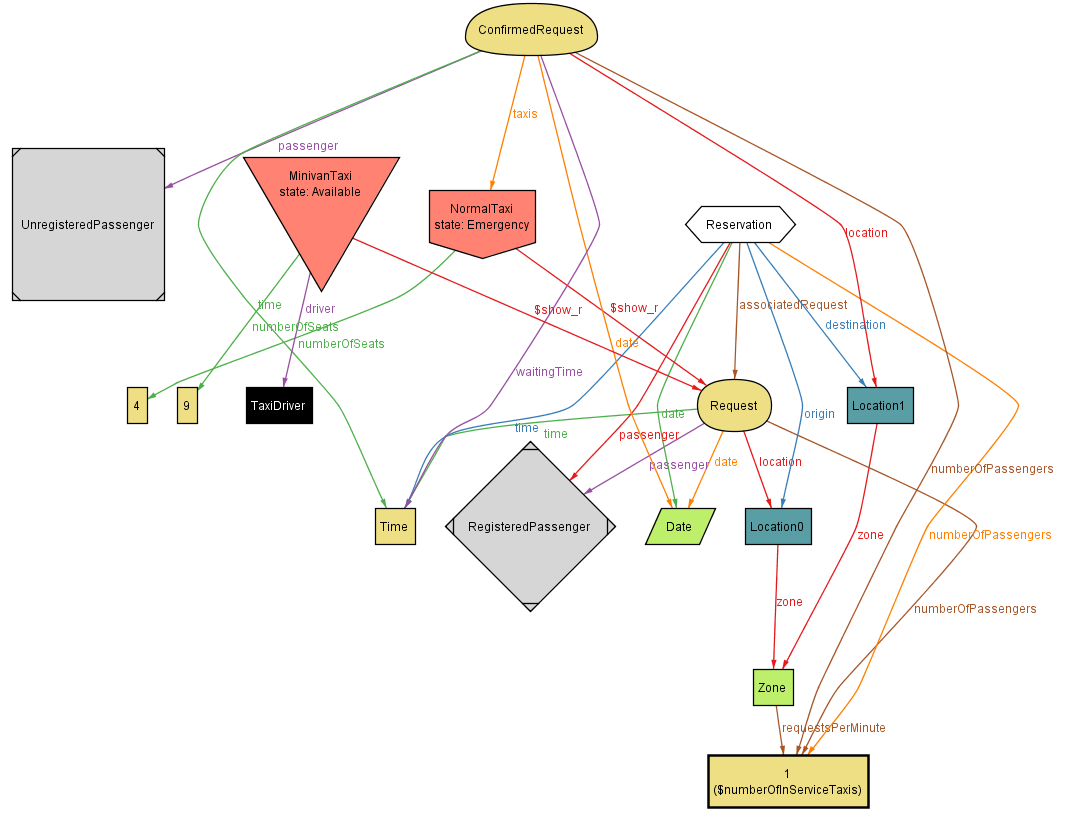
\includegraphics[scale=0.5]{alloy/instances/world1}
\par\end{centering}

\protect\caption{World generated by predicate \lstinline!pred show!}


\end{figure}


\end{landscape}

\clearpage{}

\begin{landscape}

Figure 23 is a world generated by predicate \lstinline!pred sendRequest[setOfRequests,setOfRequests': set Request, request: Request]!.
Before inserting Request2 the set of requests is composed of only
ConfirmedRequest; after the insertion also Request2 is in the set.

\begin{figure}[H]
\begin{centering}
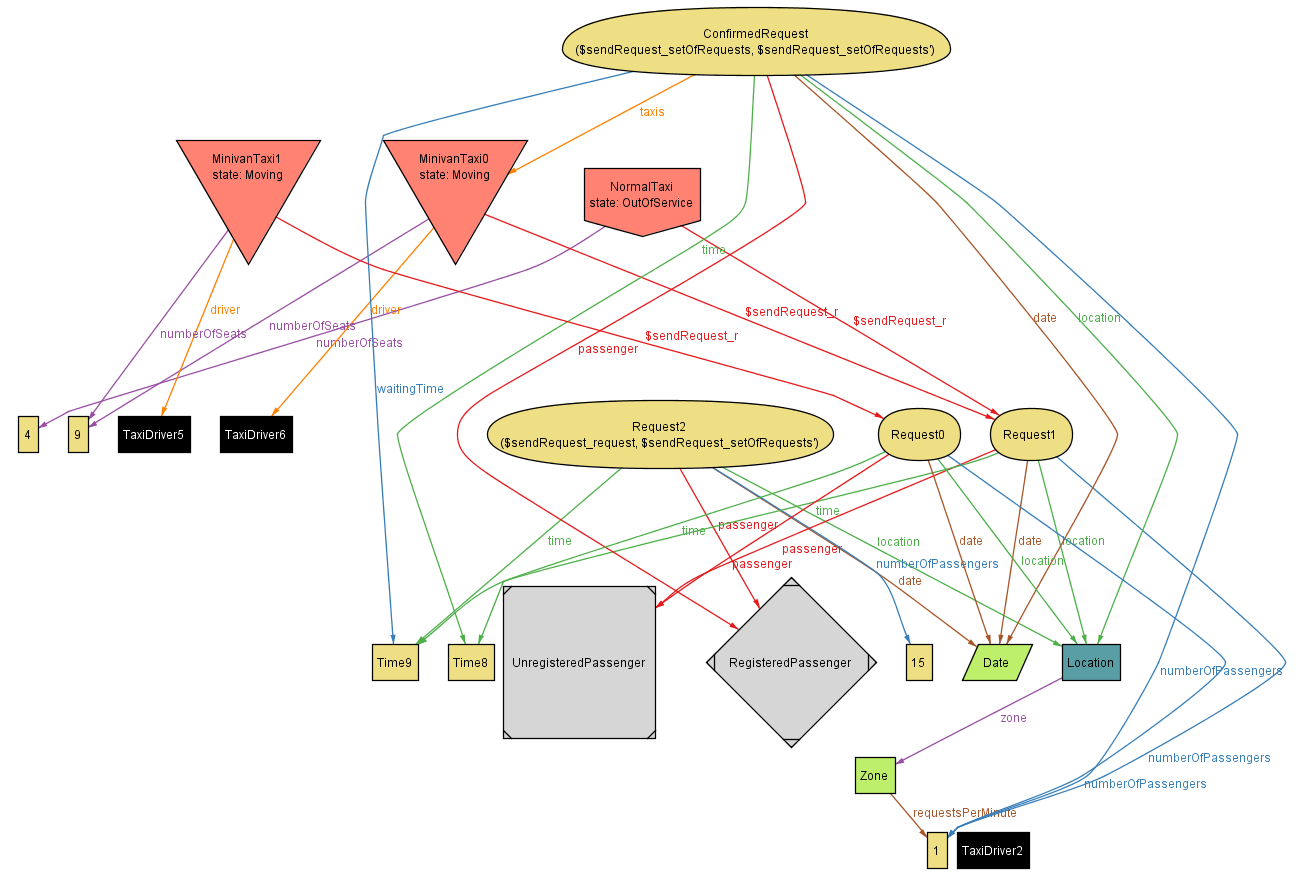
\includegraphics[scale=0.5]{alloy/instances/sendRequest}
\par\end{centering}

\protect\caption{World generated by predicate \lstinline!pred sendRequest!}
\end{figure}


\end{landscape}

\clearpage{}

\begin{landscape}

Figure 23 is a world generated by predicate \lstinline!pred sendReservation[setOfReservations,setOfReservations': set Reservation, reservation: Reservation]!.
It is clear that before the execution the set of reservation contains
only Reservation1 and after it will contain also Reservation2 (Reservation0
does not belong to any of them).

\begin{figure}[H]
\begin{centering}
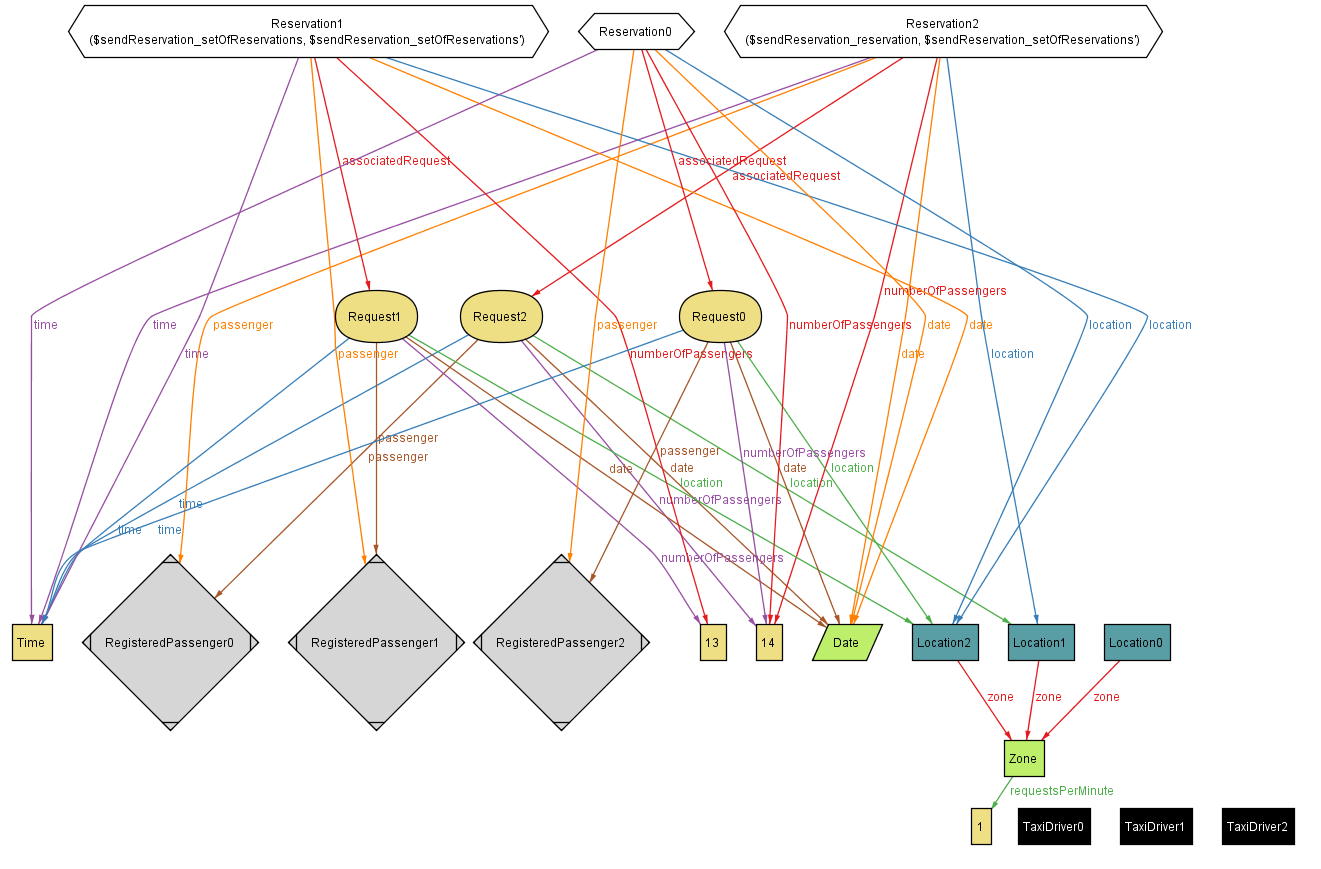
\includegraphics[scale=0.5]{alloy/instances/sendReservation}
\par\end{centering}

\protect\caption{World generated by predicate \lstinline!pred sendReservation!}
\end{figure}


\end{landscape}

\clearpage{}

\begin{landscape}

Figure 23 is a world generated by predicate \lstinline!pred cancelReservation[setOfReservations,setOfReservations': set Reservation, reservation: Reservation] !.
As you can see, before the execution Reservation1 belonged to the
set of reservation while reservation set is empty.

\begin{figure}[H]
\begin{centering}
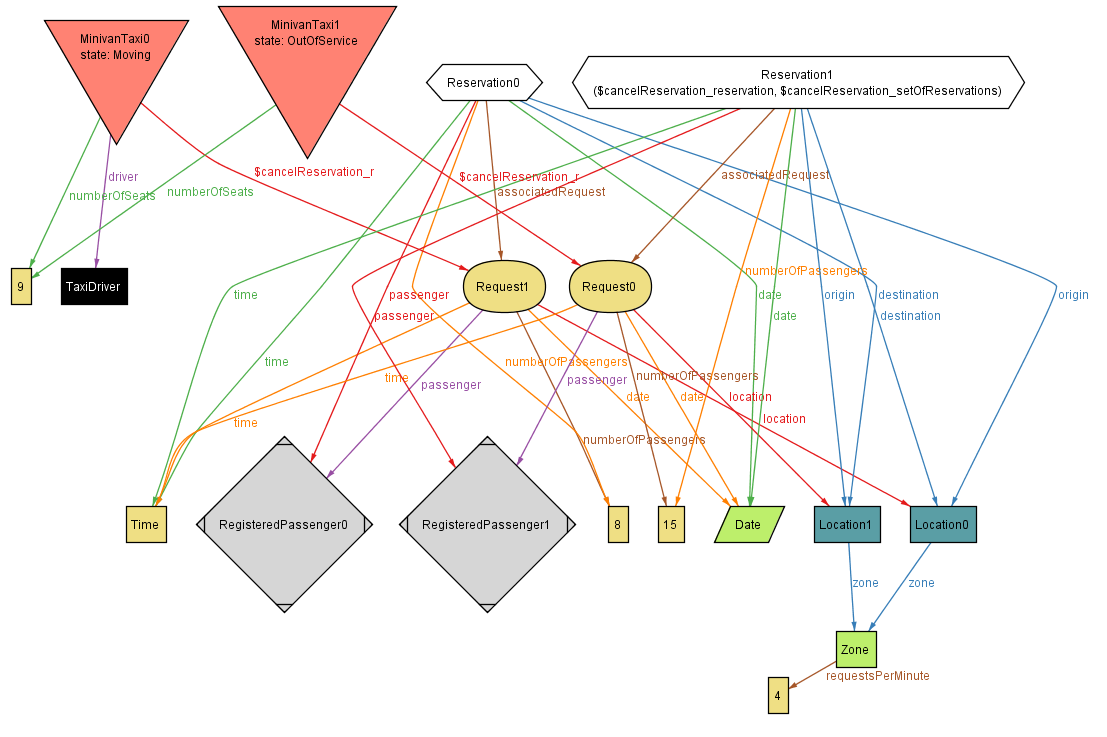
\includegraphics[scale=0.5]{alloy/instances/cancelReservation}
\par\end{centering}

\protect\caption{World generated by predicate \lstinline!pred cancelReservation!}
\end{figure}


\end{landscape}

\clearpage{}


\subsection{Queue management model}

Since queue management is a relevant part of the TS system, in this
subsection we model the structure of a queue and the adjacency relation
between zones. We will focus on the important constraints imposed
by the system but we will not model the dynamical behavior of the
queues.


\subsubsection{Signatures, facts and functions}

\begin{lstlisting}[breaklines=true]
module myTaxiService/queue

abstract sig TaxiState{} 
one sig OutOfService,Emergency extends TaxiState{} 
one sig Available, Busy, Moving extends TaxiState{}

sig Taxi { 	
	state: one TaxiState, 
}

sig Zone{ 	
	queue: one Queue, 	
	adjacentZones: some Zone, 
}

//Queue definition
sig Queue { 	
	root: lone Node 
}

sig Node { 	
	taxi: one Taxi, 	
	next: lone Node 
}

//Structural properties 
fact queueStructuralProperties { 
	
	//Each node belongs to exactly one queue 	
	all n: Node | one q: Queue | n in q.root.*next	

	//No cycles
	no n: Node | n in n.^next									 
}

//Each queue must belong to exactly one zone 
fact eachQueueBelongsToExactlyOneZone { 	
	all q: Queue | one z: Zone | q in z.queue 
}

//Adjacency relation between zones is simmetric but not reflexive 
fact adjacencySimmetricButNotReflexive 
{ 	
	adjacentZones in ~adjacentZones 	
	no adjacentZones & iden 
}

//Returns the set of taxis belonging to the queue q 
fun getTaxisFromQueue[q: Queue] : set Taxi {
	q.root.*next.taxi 
}

//Queues must store only available taxis 
fact allTaxisInQueueAreAvailable { 	
	all q: Queue | getTaxisFromQueue[q].state in Available 
}

//Each available taxi belongs to exactly one node  
	fact eachTaxiBelongsToExactlyOneNode { 	
	all t: Taxi | t.state in Available implies (one n: Node | n.taxi = t) 
} 
\end{lstlisting}



\subsubsection{Predicates}

\begin{lstlisting}
//Builds a realistic world 	
pred showQueues{ 	
	some q: Queue | #getTaxisFromQueue[q]>3 	
	some t: Taxi | t.state in OutOfService 	
	some t: Taxi | t.state in Busy 
}

run showQueues for 10 but exactly 4 Zone, exactly 10 Taxi
\end{lstlisting}


\begin{framed}
Executing "Run show for 5 but exactly 4 Zone, exactly 10 Taxi" 
Solver=sat4j Bitwidth=0 MaxSeq=0 SkolemDepth=1 Symmetry=20 
3031 vars. 176 primary vars. 6646 clauses. 15ms. 
Instance found. Predicate is consistent. 16ms.
\end{framed}


\subsubsection{Assertions}

\begin{lstlisting}[breaklines=true,showstringspaces=false]
//No available taxi are not present any queue 
assert noAvailableTaxiNotInQueue { 	
	no t: Taxi | t.state in Available and (no q:Queue | t in getTaxisFromQueue[q]) 
}

check noAvailableTaxiNotInQueue for 10
\end{lstlisting}


\begin{framed}
Executing "Check noAvailableTaxiNotInQueue for 10" 
Solver=sat4j Bitwidth=0 MaxSeq=0 SkolemDepth=1 Symmetry=20 
14039 vars. 580 primary vars. 36827 clauses. 63ms. 
No counterexample found. Assertion may be valid. 31ms.
\end{framed}

\begin{lstlisting}[breaklines=true]
//There are no taxi that appear in more than one queue
assert noTaxiSharedBetweenQueus { 	
	all disj q1,q2: Queue | no getTaxisFromQueue[q1] &  getTaxisFromQueue[q2]  
} 

check noTaxiSharedBetweenQueus for 10
\end{lstlisting}


\begin{framed}
Executing "Check noTaxiSharedBetweenQueus for 10" 
Solver=sat4j Bitwidth=0 MaxSeq=0 SkolemDepth=1 Symmetry=20 
14642 vars. 590 primary vars. 37985 clauses. 47ms. 
No counterexample found. Assertion may be valid. 531ms.
\end{framed}

\begin{figure}[H]
\begin{centering}
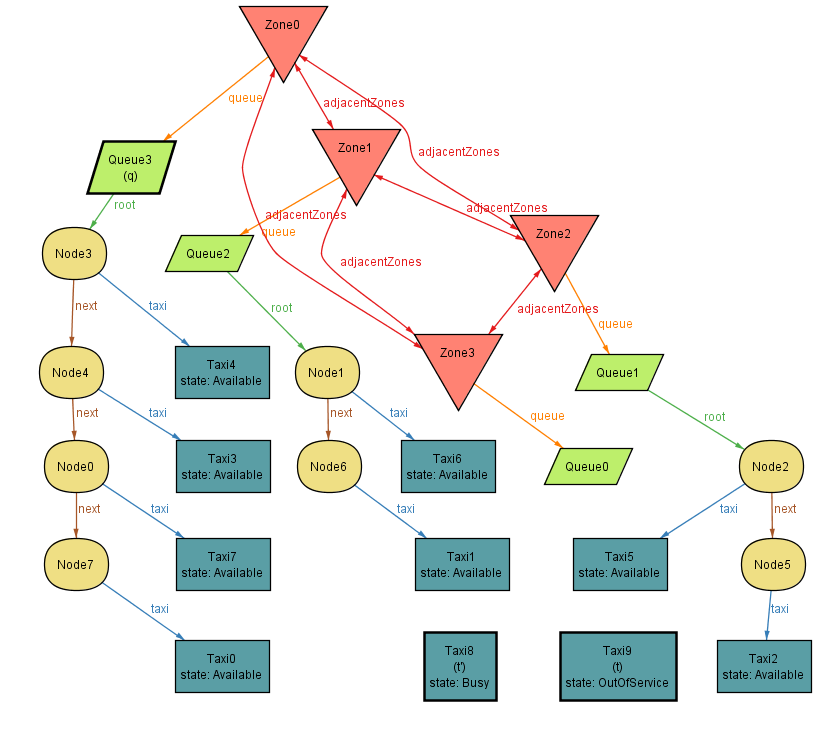
\includegraphics[scale=0.6]{alloy/instances/queues}
\par\end{centering}

\protect\caption{World generated by the predicate \lstinline!pred showQueues!}


\end{figure}



\subsection{Considerations about Alloy}

The process of modeling a complex system is always prone to many different
kinds of errors. Even though you have correctly understood the requirements
several conditions often neglected because they seem to be obvious,
but they are not. Alloy is a very precious tool that allows requirement
engineer to understand and overcome those deficiencies in the model. 
